\section{Actions as context information}
\label{sec:contribution}
In order to enhance sustainable decision-making in time evolving contexts, we strongly think that actions together with their expected effects should be part of the context representation of adaptive systems.
In this perspective, we first describe a cluster infrastructure management example for illustrating our approach.
Then, we show how an action plan can be represented as a directed acyclic graph (DAG) of actions spanned over time.
Then, we detail on how we enrich this DAG with the expected effect of actions, and later with their measured equivalences, \ie how we link the DAG to the context representation.
Finally, we illustrate how this information can be used by the MAPE-K loop to improve reasoning processes through four reasoning operations.

\subsection{Example: cluster management}
Throughout this section, we refer to a cluster management case study, the Watcher project, to exemplify our approach.
This framework performs adaptation processes over a cloud infrastructure in order to optimize resource usage, such as CPU, memory, and network. 
To achieve this, Watcher defines primitive actions to be performed, such as container's creation, migration, and duplication.
Furthermore, Watcher comes with a set of metrics, either simple or derived, for setting up optimization algorithms.
For instance, deciding whether to allocate or deallocate resources in the cluster.
In this paper, we confine to two metrics: container status and container workload.
Being part of the context information, these metrics values play a crucial role in planning and executing adaptation processes.  
These values are first modified: the system will update the container  status and their workload.
Moreover, these values can be subject to changes as a result of executing the planned actions. 

A common adaptation scenario is minimizing the amount of resources provided by
the cluster to answer a given service workload ($W_S$) that is expected a priori.
The framework thus has to decide whether to allocate or deallocate resources, and thereby, increase or decrease the amount of the provided workload ($W_P$). 
To do so, the framework first compares $W_S$ to $W_P$, then determines the most convenient action plan. 
As soon as an allocation or deallocation action is performed, the workload values are increased or decreased and the container statuses are modified accordingly (e.g., \textit{READY}, \textit{DOWN}).
Neither of these actions is effective immediately and they can be subject to failure.
As shown in~\cite{DBLP:conf/IEEEcloud/MaoH12}, a virtual machine based on Linux could take from 90 seconds to more than 200 seconds to be ready. 


\subsection{Action planning}
\label{sec:contribution-dag}

System adaptation is commonly performed as a set of actions. 
In complex scenarios, these actions are often interdependent and require advanced action planning.
It takes into consideration not only dependency but also actions execution status. 
Furthermore, existing simplified models,\eg~\cite{7194653,5984008}, do not capture action execution time and assume that they complete immediately after they are triggered. 
Capturing such temporal information (\eg (de)allocation delays) contributes to the quality of context information and improves the reasoning process of the MAPE-K loop.

We propose to represent action plans by means of DAGs of actions spanning over time,  where each node corresponds to an action and an edge to a precedence relationship between actions. 
Figure~\ref{fig:action_dag} shows an example of an action plan represented using an actions DAG.
Actions can be executed in parallel or sequential way.
Each action has a \textit{start time}, an \textit{execution duration}, and \textit{a time until its effects are measurable} by the system.
These properties can be reproduced using the three temporal functions defined in Section~\ref{sec:temporal_model}.
The execution duration will be the difference between the \textit{start time} and the \textit{end time} values, defined by the \textit{start(id)} and \textit{end(id)} functions.
Expected effects resulting from the execution of an action are also attached to actions, as highlighted in  Figure~\ref{fig:action_dag} by a dashed arrow. 
The \textit{ time until action effects are measurable} will correspond to the start time, \ie the result of the function \textit{start(id)}, of the context element.
We differentiate between several actions statuses, namely, created, pending, running, failed, succeeded, or canceled.
An action is triggered when all the actions of the incoming edges succeed. 
In case of actions failure or cancellation, the subsequent actions are canceled then rescheduled for the next planning phase. 
We provide more details about expected effects representation below.
This DAG is then fed to the knowledge component of the MAPE-K feedback loop to improve the reasoning process.

We describe in the next section how we represent this DAG and how we link it to the context presentation.

\subsection{Linking action planning and context representation}


In order to enable reasoning on actions, we include two concepts in our context representation model, the \textit{measured} value and \textit{expected} value.
While \textit{measured} represents the value of data measured by the system's sensors, \textit{expected} represents data reflecting the planned effects of actions.
We assume that actions are triggered by change requests made either by a human or the system itself (\eg the reasoning process).
Based on change requests, the reasoning process will generate the DAG of actions with effects on metrics.
For the sake of understandability, this concept should encapsulate the intent behind performing an action.

An excerpt of a meta-model representing these concepts is provided in Figure~\ref{fig:mm_contrib}.
The right-hand side of the meta-model depicts how we model change requests, thanks to the \textit{ChangeRequest} meta-class.
The \textit{name} and the \textit{type} are used by the reasoning process to infer the desired state as well as the actions to reach it.
The \textit{timeLimit} attribute allows to define a time-out for each individual request.

The center part of the meta-model (with grey background) depicts the meta-model used to create instances of the DAG of actions. 
To support the sequential and parallel execution, we define three classes: \textit{Action}, \textit{Fork Action} and \textit{Join Action}.
While sequential actions can be modeled using the relationship \textit{next}, parallel nodes can be modeled using fork actions and join actions.
The \textit{JoinAction} is simply a node with multiple incoming edges, while the \textit{ForkAction} node with multiple outgoing edges.
The actions are part of the context model thanks to the reference \textit{next} associating the \textit{Action} class to the \textit{ContextModel} class.

The left-hand side deals with the sub-model that supports expected effects.
A value of a metric can be of any type. 
We represent it in the metamodel through the generic type parameter \textit{T}.
Metrics with \textit{measured values} are directly connected to the context model.
This corresponds to the usual semantics of context models.
In the Figure~\ref{fig:mm_contrib}, this is shown by the \textit{Metric} class.
\textit{ExpectedMetric} are used to represent the expected values.
Thanks to the \textit{timeDephasing} and the \textit{precision} attributes we are able to handle time expressions with a high level of precision.
Conceptual links between an action and its corresponding expected metrics are established using the relationship \textit{effects} (depicted in bold red). 
Using this representation, we enable the analysis using expected values, measured values, actions, and their effects. 
As we will show in the next section, this representation improves significantly the analysis and planning phases of traditional MAPE-K loops. 
%In the next section, we introduce a cloud electricity manager case study to demonstrate our approach on a concrete case study, before we present reasoning abilities thanks to our approach.

\begin{figure*}
	\centering
	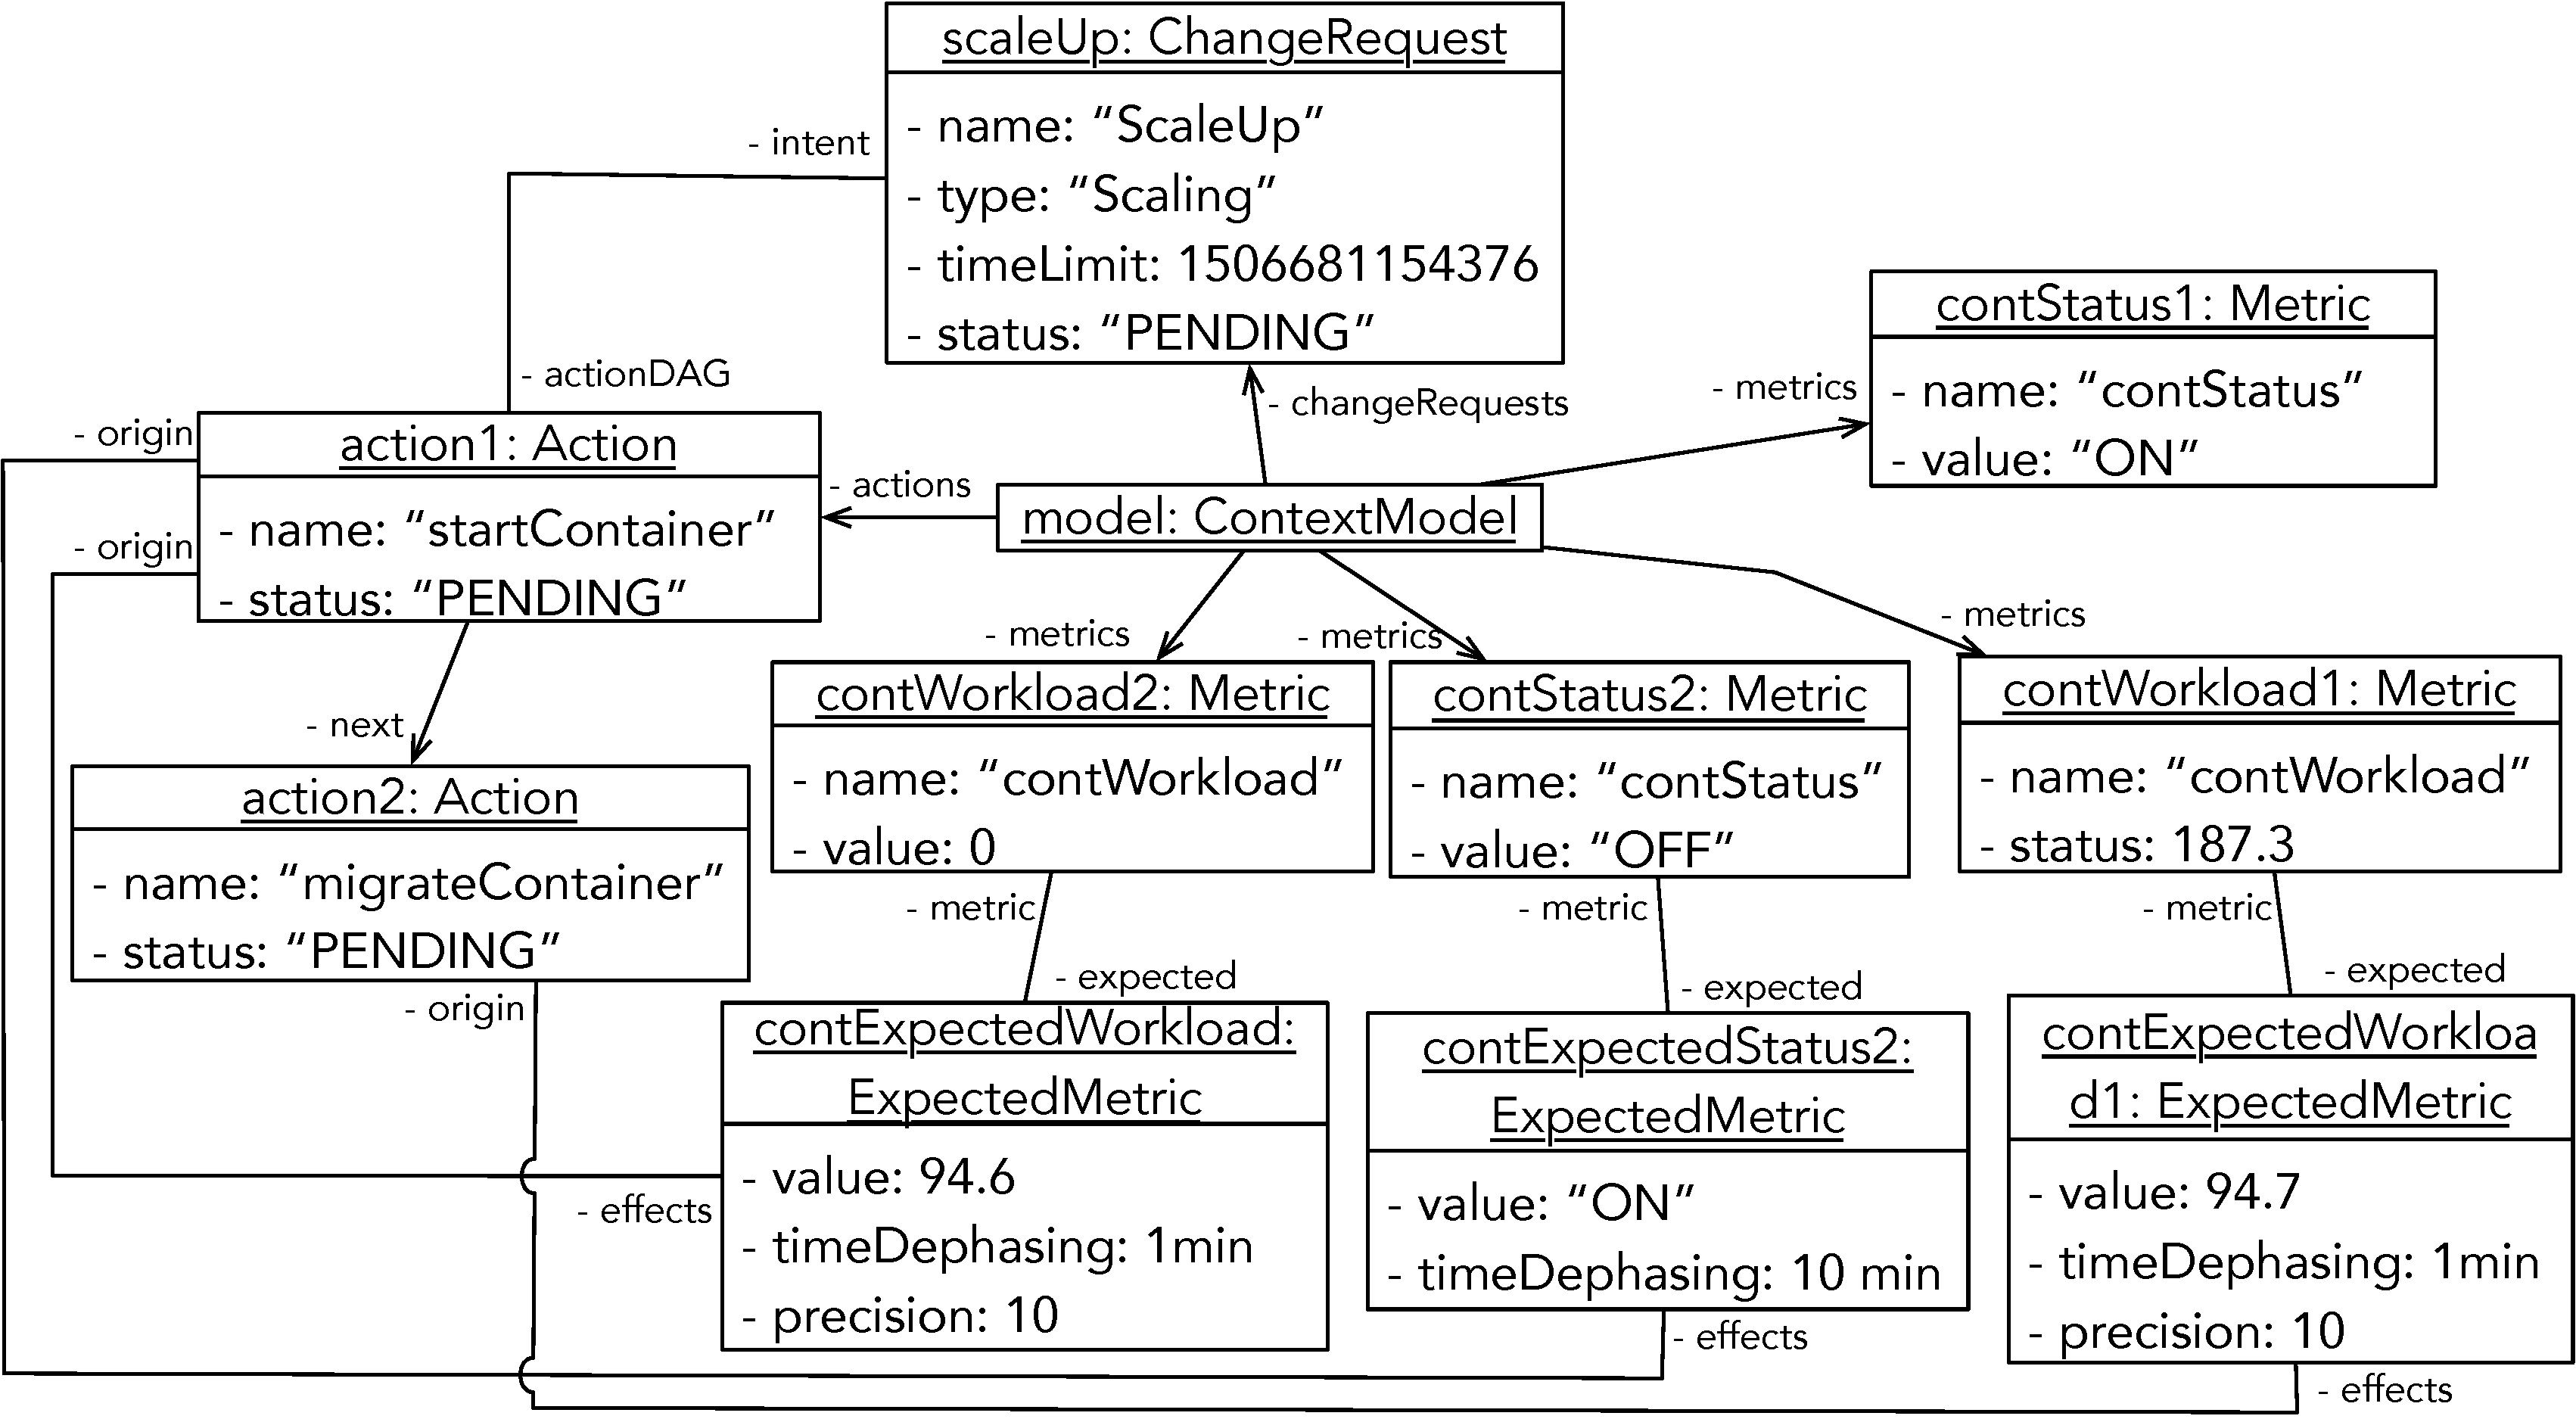
\includegraphics[width=0.7\linewidth]{img/chapt-tkm/actionAsContextElement/example2}
	\caption{Instance model of the cluster management use cases.}
	\label{fig:example-complete}
\end{figure*}

Coming back to our case study, Figure~\ref{fig:example-complete} depicts a model instance of our proposed example.
The meta-model contains four metrics: container status (\textit{contStatus1} and \textit{contStatus2}) and container workloads (\textit{containerWorkload1} and \textit{containerWorkload2}).
All these metrics are affected by two actions: \textit{action1}, an action to switch a container on, or \textit{action2}, an action to migrate a container to another host.
As a scale up request has been created, the reasoning process decides to create an action plan: first switching a container on and then migrating another container.

\subsection{Enabled reasoning} 

By associating the action model to the context model, we aim at enhancing adaptation process with new abilities to reason.
In this section, we list four kinds of reasoning that is possible thanks to our approach: (i) answering change requests (ii) immediate supervision, (iii) future supervision, (iv) meta supervision.
We also present the necessary code to extract information during the reasoning phase.
We use a dot notation for navigating inside our context model, \ie for accessing the properties (attributes and relationships).
Moreover, we consider the elements as stream, \ie each context elements are contained in a stream of elements.
For example, the metrics are contained in a stream of context elements. 
In addition, context elements define the same operation as the ones of the Stream Java interface\footnote{https://docs.oracle.com/javase/8/docs/api/java/util/stream/Stream.html, Last visited: 28 September 2017}.
The execution semantics also remains similar.
When the operations are executed, they are executed at a precise time, \ie the current timestamp.
When operations need to access a context element, they apply the \textit{resolve(id,time)} functions as described in Section~\ref{sec:background}.
For readability purpose, we do not show the call to this function.
Listed codes have been made using the context model presented in Figure~\ref{fig:example-complete}.


\paragraph{Answering change requests}
Thanks to change requests present in the context representation, the reasoning will create a DAG of actions to reach a desired state.
It thus needs to extract the change requests that have not been processed and on which the time limit has not been reached. 
If the time limit has been reached or overtaken, the reasoning process could throw errors.
We present the code to extract the change requests from our model in Listing~\ref{code:ansewring-requests}.

\begin{figure}
\begin{lstlisting}[style=customc,caption=Generation of the DAG of actions from the change requested,label=code:ansewring-requests,basicstyle=\scriptsize]
model.changeRequests
     .select(ChangeRequest cr -> cr.status == "PENDING")
     .select(ChangeRequest cr -> cr.timeLimit <= NOW})
     .forEach(ChangeRequest cr -> createActions(cr))
 
//Rise an error for unsatisfied requests
model.changeRequests
     .select(ChangeRequest cr -> cr.status == "PENDING")
     .select(ChangeRequest cr -> cr.timeLimit > NOW)
     .forEach(ChangeRequest cr -> riseError(cr))
\end{lstlisting}
\end{figure}


\paragraph{Immediate Supervision}

When a reasoning process plans adaptation actions, it also sets the expected effect on the metric of the context model. 
We refer to this operation as immediate supervision. 
However, the measured value could diverge from the expected one for different reasons: error in actions, context that has not changed as expected, or wrong effect extrapolation.
The reasoning process needs to detect this divergence for taking counteractions.
In other words, the reasoning process needs to analyse the difference between the expected value and the measured one.
We present the code to achieve the extraction of the expected and the measured value of a metric in Listing~\ref{code:supervision}.
As shown in the code, the checking should consider both the precision of the expected value and the possible temporal dephasing between the measured value and the expected effects. 
We check if the value is in the following range:  $[effect value - precision ; effect value + precision]$ and the time of the measured value is the following range: $[time - time dephasing; time + time dephasing]$.

%\begin{figure}[ht!]
\begin{lstlisting}[style=customc,caption=Detection of difference between measured and expected values, label=code:supervision, basicstyle=\scriptsize]
model.metrics
     .select(Metric m -> m.name == "contWorkload")
     .forEach(Metric m -> { 
     	 ExpectedMetric e = m.expected;
     	 if(m.value < e.value - e.precision || 
     	    m.value > e.value + e.precision) {
     	     if(time(m.id) < start(e.id) - e.timeDephasing || 
     	        time(m.id) > start(e.id) + e.timeDephasing) {
     	          createCorrectiveActions(m); }
         }
     })
\end{lstlisting}
%\end{figure}


\paragraph{Future supervision}
Actions are taken for adapting the system to the current context.
However, they are not immediately and successfully executed and their effects are measurable with delay.
As discussed in Section~\ref{sec:introduction2}, the reasoning frequency could be inferior to this delay.
It results on a reasoning process that will be executed on a similar context as the last execution.
It will thus take the same action(s) whereas the context will be adapted soon.
To tackle this problem, using our approach, the reasoning process can also consider the future expected metrics.
By analysing the current context for detecting any miss adaptation and the future expected one for detecting any future correction, the adaptation process will avoid repetition of actions.
The code below show how to extract the current container workload and the future expected one.
The code remains similar to the previous one (Listing~\ref{code:supervision}) except that we resolve the expected value at another time, here 5 min after the current time (\textit{NOW}).

\begin{lstlisting}[style=customc,caption=Extraction of expected and measured value of a metric with a delta time,label=code:supervision-future,basicstyle=\scriptsize]
model.metrics
     .select(Metric m -> m.name == "contWorkload")
     .forEach(Metric m -> {
         ExpectedMetric futureE = resolve(m.expected,NOW + 5min)
         //similar to the code presented in Listing 1
      })
\end{lstlisting}

\paragraph{Meta supervision}

Supervision allows to verify that the reasoning has been successfully executed, \ie that the expected effect really happened on the system.
As explained in the previous paragraph, the system will also diverge from this desired state for different reasons.
The meta supervision aims at finding extra information.
For example, we will detect if a desired state is not reachable, or that an action often creates this divergence.
The code presented in Listing~\ref{code:meta-supervision} allows to detect actions that did not achieve the expected effect.
For this purpose, we check if an action did not surpass the expected percentage \textit{THRESHOLD} of miss expectations.

\begin{figure}[ht!]
\begin{lstlisting}[style=customc,caption=Extraction of expected and measured value of a metric with a delta time,label=code:meta-supervision,basicstyle=\scriptsize]
Map<Action,Integer> error= new HashMap();
int sum = 0;

model.timeRange(NOW - 2H, NOW)
     .metrics
     .forEach(Metric m -> {
        [...] //code of previous listing
        if(...) {// if presented in the previous listing
            Action a = m.expected.origin;
            int count = error.get(a) + 1; 
            error.put(a, count);
            sum++;
        }
      });

error.forEach((key,value) -> {
         if(value / sum > THRESHOLD) {
            takeActions();
         }
    });
\end{lstlisting}	
\end{figure}
